\chapter{\acs{lidar} Interference}
\label{chapter:lidar-interference}

\ac{lidar} interference is occurs when the signal of one \ac{lidar}, ``A'', interferes with the signal of another \ac{lidar}, ``B'', affecting its measurements, i.e., the \ac{lidar}'s ``B'' capability to measure the distance what which is laser pulse was reflected is not independent of the presence of another \ac{lidar} on its surroundings. On telecommunications, when two devices on the same channel or physical environment interact, creating an undesirable effect with negative consequences, we are in the presence of crosstalk. On the \ac{lidar} interference scenario, this interference can be direct or indirect (the beam is reflected on other surface(s) before hitting the \ac{lidar} ``B'').

The main goal of this thesis is to research the \ac{lidar}'s interference behavior, expanding the previous work, presented on the Section~\ref{sec:sota:lidar-interference}. \acl{sota} on \ac{lidar} interference is still reduced, with the major contributions from only two research teams, and for an experimental setup with only two-dimensional \acp{lidar}, i.e., rotating \acp{lidar} that can scan a single line from the environment.

On this chapter, we start by explaining the additions to the previously described experimental setup, on Section~\ref{sec:calibration:experimental-setup}, that allows us to investigate the impact of several parameters on \ac{lidar} interference behavior. Experimental test scenarios are detailed and the test conditions under which data was acquired are explained. Since one of the thesis objectives, detailed in Section~\ref{sec:introduction:objectives}, is to create a comprehensive experimental dataset, with different metrics, for future tests on \ac{lidar} interference, we present how the experimental dataset was organized to ensure it could be easily reused but also to streamline data analysis on this research.

Our first \ac{lidar} interference analysis results are obtained from Bosch\cp~datasets, allowing a qualitative assessment of the interference. Based on these results, we sought to explain this behavior by quantifying the number of outliers that have no physical context on the data, such as points below ground or outside a closed room dimensions.

To provide a more in-depth analysis of the interference, a comparison with a ground-truth model of the test environment is required. Therefore, we propose two methods to generate such ground truth model from the data without interference. Using these models, we also propose two methods to measure the interference, unveiling their algorithms and results.

Following up on the outcomes provided by Chapter~\ref{chapter:object-detection}, we apply the previous algorithms onto the selected \acp{roi} on the point cloud, that correspond to the bounding boxes of image objects previously detected on the image, using the calibration notions gathered from Chapter~\ref{chapter:calibration}.

Lastly, we conclude our findings and compare them with the current \acl{sota} on \ac{lidar} interference.

\section{Experimental Setup}
\label{sec:lidar-interference:experimental-setup}

Expanding the previous experimental setup, detailed in Section~\ref{sec:calibration:experimental-setup}, requires adding another \ac{lidar}, that acts as an interferer. This \ac{lidar} is mounted on a tripod and serves the purpose of interfering with the measurements of the first \ac{lidar}, already present on the earlier version of the experimental setup (see figure~\ref{fig:experimental-setup}), which becomes its ``victim''\footnote{The terms victim and interferer, when referring to \ac{lidar} interference, are first connoted by Gunzung Kim\etal on~\cite{Kim2015a, Kim2015b, Kim2015c, Kim2017}, and later adopted by Gerald Popko\etal~\cite{Popko2019a, Popko2019b}. To keep the notation coherent with the \acl{sota}, we will use the same denominations on this chapter.}.

The interferer \ac{lidar} is a HESAI\cp~Pandar40\texttrademark, a 40 beams \ac{tof} \ac{lidar} that operates at a frequency of \SI{905}{\nano\meter}. Pandar40 supports various measurements modes based on the return pulse (Strongest, Last, Dual) and can be connected to a \ac{gps} receiver for geopositioning and synchronization with an external clock. It also supports two rotation velocities: 600 or 1200 \ac{rpm}, which result in different angular steps and point cloud refresh rate. 

Pandar40's \ac{lidar} has an asymmetrical vertical \ac{fov}, varying from \SIrange{-16}{+7}{\degree}. A larger channel density occurs between the angles \SI{-6}{\degree} and \SI{+2}{\degree}, with 25 pairs of lasers and photoreceptors with \SI{0.33}{\degree} apart from each other. From \SIrange{-16}{-6}{\degree} and \SIrange{+2}{+7}{\degree}, the angular step between the pairs of lasers and photoreceptors is \SI{1}{\degree}, and only 15 pairs of lasers and photoreceptors are used: 5 above and 10 below.

The full specifications of the HESAI Pandar40 can be accessed on~\cite{Pandar40UserGuide} and the relevant specifications for this work are summarized on table~\ref{tab:pandar40-specs}.

\begin{table}[H]
	\centering
	\renewcommand{\arraystretch}{1.2}
	\rowcolors{3}{gray!10}{white}
	\begin{tabular}{@{}p{6cm}c@{}}
		\toprule
		Specifications & Value \\
		\midrule
		Wavelength & \SI{905}{\nano\meter} \\
		Motor \ac{rpm} & 600 \\
		Angular Step & \SI{0.2}{\degree} \\
		Vertical \ac{fov} & \SI{23}{\degree} \\
		Horizontal \ac{fov} & \SI{360}{\degree} \\
		Maximum Scanning Distance & \SI{200}{\meter} @20\% reflectivity \\
																					 & $\pm \SI{5}{\centi\meter}$, from \SIrange{0.3}{0.5}{\meter} \\
		\rowcolor{white} \multirow{-2}{*}{Measurement Accuracy} & $\pm \SI{2}{\centi\meter}$, from \SIrange{0.5}{200}{\meter} \\
		\bottomrule
	\end{tabular}
	\caption{HESAI Pandar40 relevant specifications. Source~\cite{Pandar40UserGuide}.}
	\label{tab:pandar40-specs}
\end{table}

The tripod used for the experimental setup is a Velbon\cp~CX-460\texttrademark~tripod, that also has a central monopod. For increased stability on the measurement procedure, the monopod was never used. The tripod ranges in height from approximately \SIrange{0.62}{1.28}{\meter}, measured from its feet to its basis. Since the tripod used is a camera tripod, a gimmick must be done to ensure proper fixation of the Pandar40 \ac{lidar}, by replacing the universal camera support bolt with an \SI{12}{\milli\meter} length M6 bolt, tighten with a M6 nut and two metal rings. The Pandar40, secured on the tripod, is shown on figure~\ref{fig:pandar40-on-tripod}.

\begin{figure}[H]
	\centering
	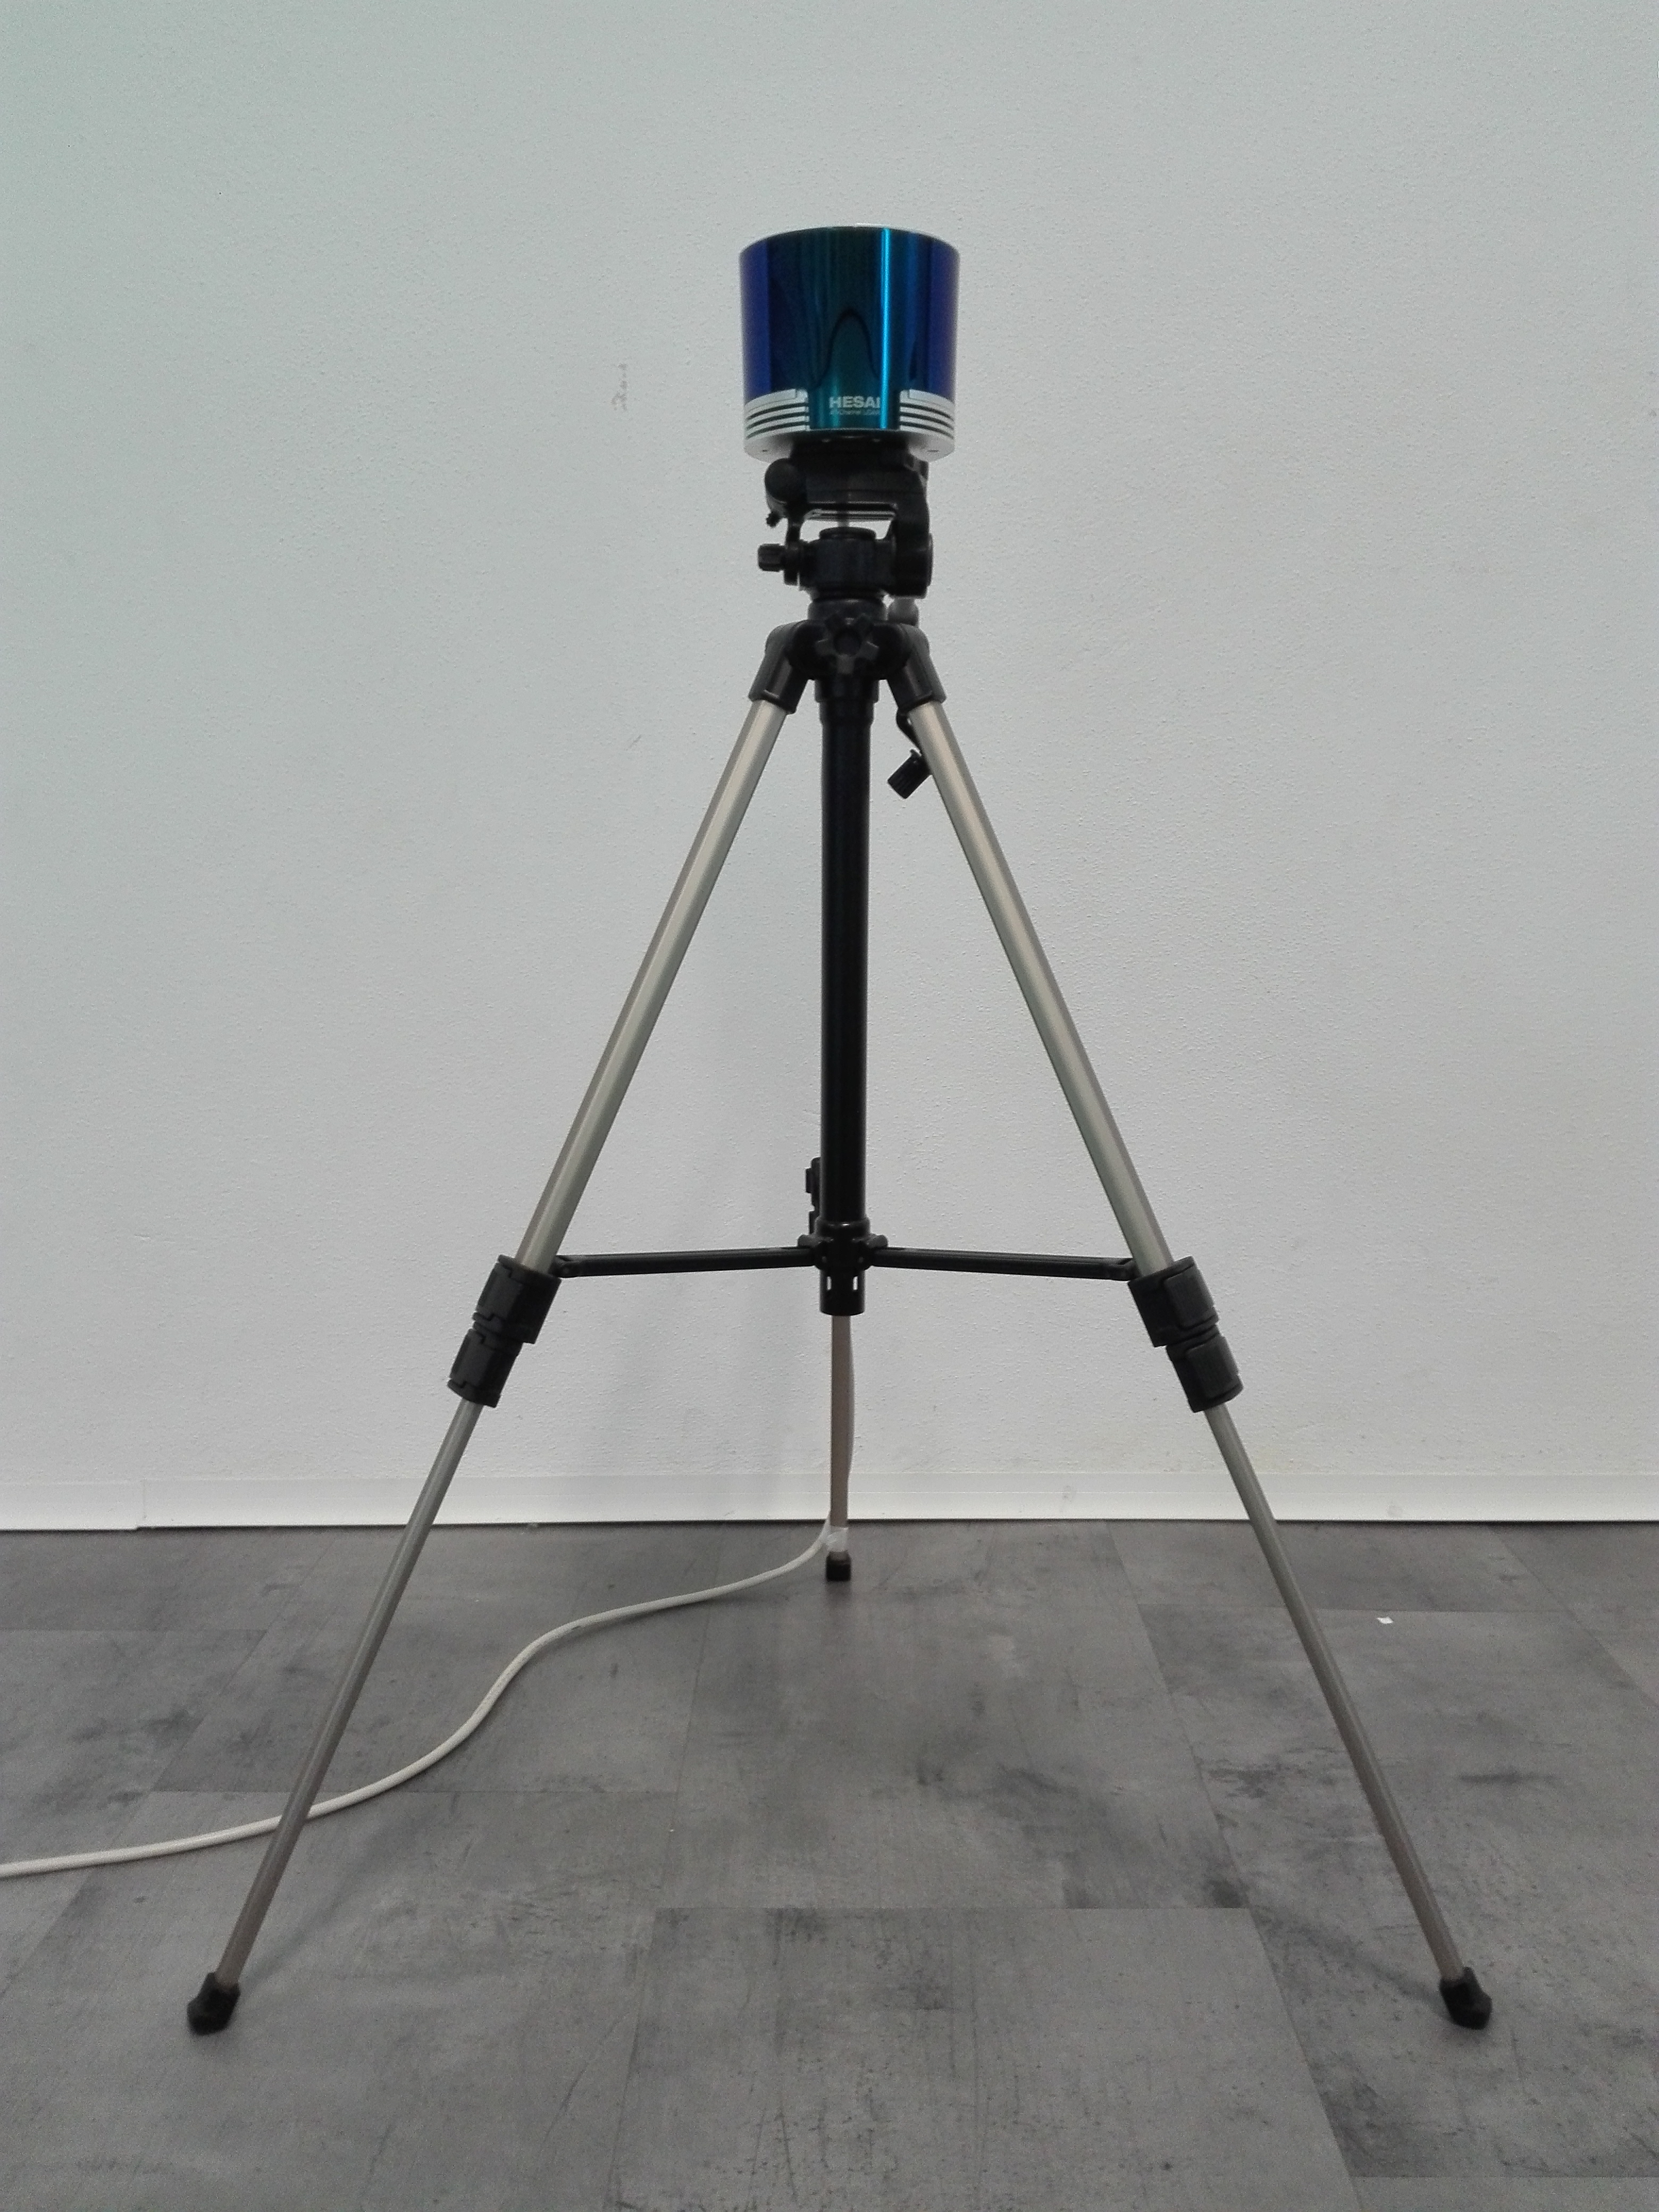
\includegraphics[width=0.4\textwidth]{img/experimental-setup/pandar40-on-tripod.jpg}
	\caption{HESAI Pandar40 \ac{lidar} on a Velbon CX-460 tripod.}
	\label{fig:pandar40-on-tripod}
\end{figure}

Despite the two \acp{lidar}'s laser nominal frequencies not being equal, no majors drawbacks are expected due to the mismatch. Velodyne's VLP-16, the victim, operates at \SI{903}{\nano\meter} and HESAI Pandar40, the interferer, operates at \SI{905}{\nano\meter}. Ideally, the same \ac{lidar} model would be used for the victim and interferer, but such material was not available. Nevertheless, we are unable to predict how the different number of channels, asymmetric channel distribution, variable angular step and different laser wavelength will impact the interference behaviour, due to the lacking of prior knowledge available on the area.

\subsection{Experimental Test Scenarios}
\label{subsec:lidar-interference:test-scenarios}

Two places were used as test scenarios for \ac{lidar} interference: Aveiro's \ac{it} Dark Room and \ac{irislab} \ac{msl} robotic soccer field. On the former, acquaintance with the experimental setup, calibration procedures and tests to gathered preliminary knowledge on \ac{lidar} interference were carried. On the latter, experimental tests were devised to research the impact of relevant parameters under study on \ac{lidar} interference. 

Aveiro's \ac{it} Dark Room is an optical laboratory that is capable of blocking all external light (hence its name). It measures $\SI{5.20}{\meter} \times \SI{6.97}{\meter} \times \SI{2.80}{\meter}$ and is equipped with desks, chairs, optical experimental setups, among other things, creating a noisy scenario for a \ac{lidar} rangefinder. 
\ac{irislab} \ac{msl} robotic soccer field measures $\SI{18.0}{\meter} \times \SI{11.5}{\meter}$ and is placed inside \ac{irislab} building, a research facility whose main division has $\SI{34.346}{\meter} \times \SI{16.097}{\meter} \times \SI{4.289}{\meter}$, if measured to the ceiling and not the ceiling girders. 

All distance measures presented on this Chapter are taken using LOMVUM LV66V \SI{80}{\meter} laser rangefinder. When taking measures, the orientation of the rangefinder was kept in the interval of $[\SI{-0.2}{\degree}, \SI{0.3}{\degree}]$. The error associated to each laser measurement, according to LOMVUM datasheet\footnote{No online manual was found. Measurement error determined by consulting the product printed datasheet, supplied with the device.} is \SI{1.5}{\milli\meter}. To minimize the error introduced by the human operator, 10 measurements were done and their average was taken, considering it the value that is represented, using the LOMVUM's laser rangefinder capabilities.


\subsection{Parameters under study}
\label{subsec:lidar-interference:parameters-under-test}
On \ac{irislab}, several tests were devised to tackle the problem of \ac{lidar} interference from different perspectives. Tests scenarios were carried, where only one parameter is varied, in an attempt to understand the interference behavior between data. The test parameters under studied, from which different datasets were recorded are:

\begin{itemize}
	\item \textbf{Distance:} Keeping the \acp{lidar} azimuthal origin aligned and with their focal center at the same height, the distance between the interferer and victim is changed, by moving the interferer further away. The distance between the two was varied in steps of \SI{1}{\meter}, from \SIrange{1}{12}{\meter};
	\item \textbf{Height:} For a fixed distance between the two \acp{lidar}, with its azimuthal origin aligned, the height between the two is varied in non-uniform steps, from \SIrange{0.623}{1.277}{\meter} measured in relation to the floor, which results in \SIrange{-0.295}{0.359}{\meter} when compared with the victim \ac{lidar} height;
	\item \textbf{\acp{lidar} \ac{los} obstruction:} To quantify the impact of direct and indirect interference, an obstacle is placed on the \acp{lidar} \ac{fov}, breaking the \ac{los} between the two \acp{lidar} This test scenario places the interferer at the even distances from the distance test, with the obstacle placed at the middle distance between the victim and interferer \ac{lidar}. The remaining test conditions are similar to the Distance tests;
	\item \textbf{Rotation Speed:} To measure the impact of different rotation speeds between the \acp{lidar}, the victim's \ac{lidar} is kept at the same rotation speed as the other tests, while the interferer \ac{lidar} rotation speed is changed. Distance is constant, the \ac{lidar}'s azimuthal origin is aligned and their focal length is at the same height;
	\item \textbf{Orientation:} To study the interference directionality, the relative angular position between the victim's and the interferer \ac{lidar} is changed, while keeping their focal length at the same height and the same distance for all variations of this parameter.
\end{itemize}


\subsection{Dataset Organization}
A thesis objective on its own (see Section~\ref{sec:introdcution:objectives}), dataset organization is a crucial for a proper data analysis. With 5 parameters under test, each with several values, 60 different interference test exists, in addition to camera calibration data and data without interference. On total, more than \SI{600}{\giga\byte} of pre-processed raw data, ready to be analyzed, is stored, in a total of almost 180 \ac{ros} bag files, totalling almost 4 hours and 20 minutes of playable data. Several hundred files, among camera calibration, rigid body transform and results, are also contained on the dataset structure, for a total of more than \SI{1}{\tera\byte} of data and results.

A comprehensive diagram that details the dataset directory and file tree hierarchy for data recording is given on~\nameref{appendix:datasets-tree}. The \textit{Experimental Datasets} folder is the root folder of the data, containing the two test locations, \textit{IRIS Laboratory} and \textit{IT2 Dark Room}. 

The standardization of tests scenarios started on \ac{it} 2 Dark Room, but only matured on \ac{irislab}. This standardization forces guidelines on file and folder naming, directory structure organization and data to record. On every folder, a \textit{README.md} file is present, detailing the files and/or folders in its hierarchy level, and the test conditions, if applicable. 

On \ac{it} 2 Dark Room, only \textit{Scenario B} follows these guidelines, which were inspired by \ac{kitti}'s dataset~\cite{Geiger2013a}. Since our setups location is fixed, each location defines a root folder for all the tests happening in that location, with its subfolders being the day on which the data was acquired. These type of folders contain  3 subfolders, whose goal is detailed below and an extract of its  hierarchy organization is given on figure~\ref{fig:test-subfolders}.

\begin{figure}[H]
	\centering
	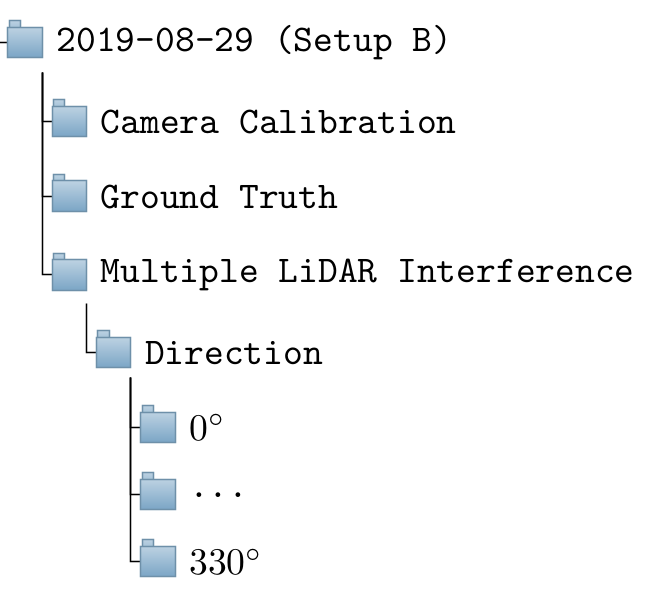
\includegraphics[scale=0.3]{img/datasets/test-subfolders.png}
	\caption{Detail of the hierarchy of a ``test day''. On each day data was recorded, calibration and ground-truth data were recorded. \textit{Multiple Lidar Interference} folder contains the parameters under test and each of the tested values.}
	\label{fig:test-subfolders}
\end{figure}


\begin{enumerate}
	\item \textit{Camera Calibration}: Contains the calibration images, intrinsic calibration parameters, \ac{ros} bag files containing the camera and \ac{lidar} raw and pre-processed data and the log file of the calibration procedure;
	\item \textit{Ground Truth}: One or more \ac{ros} bag file containing the static scenario, without objects of interest placed on the camera's and \ac{lidar} \ac{fov} and without \ac{lidar} interference;
	\item \textit{Multiple LiDAR Interference}: This folder contains a series of subfolders, each for a parameter under test. For each parameter under test folder, subfolders contain the data and results for each of the value that the parameters takes.
\end{enumerate}

On a specific value for a parameter under test, three bag files are present, as shown in figure~\ref{fig:parameter-test-files}. \textit{interference.bag} is a pre-processed \ac{ros} bag file that contains only \ac{lidar} data with interference. This pre-processing consists on cropping the \textit{original\_raw.bag} file to remove the initial seconds (from \SIrange{20}{30}{\second}), when the interferer \ac{lidar} is still booting up. \textit{ground\_truth} corresponds to data recorded under the conditions of \textit{interference.bag}, but without interference, i.e., the interferer \ac{lidar} is its position for the test, but switched off.

\begin{figure}[H]
	\centering
	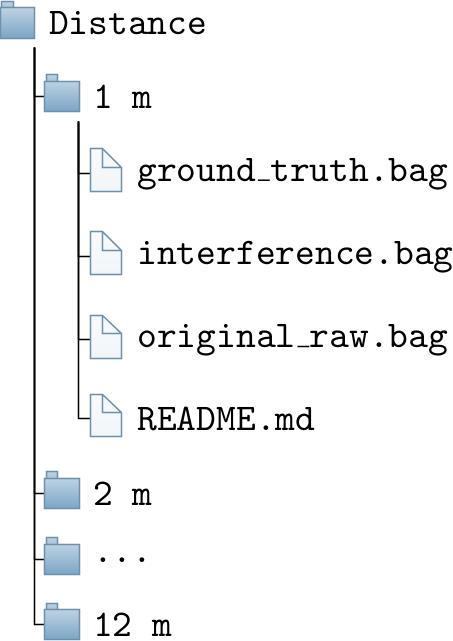
\includegraphics[scale=0.3]{img/datasets/parameter-test-files.png}
	\caption{Data recorded using \texttt{rosbag} tool, for a single value of a parameter under test. \textit{README.md}, on this type of folder, details the conditions under which data was gathered.}
	\label{fig:parameter-test-files}
\end{figure}


On \textit{IRIS Laboratory} folder, two test folders are present, containing all the data gathered on \ac{irislab}, \textit{2019-08-28} and \textit{2019-08-29}. For each of the folders, different calibration parameters are available, along with ground truths and calibration data. For \textit{\ac{it} 2 Dark Room}, only the data on the folder \textit{2019-07-31} is relevant to interference analysis.

To ease the access to this data structure, \texttt{datasets\_path} library was implemented, both on C++ and Python 3, to allow ubiquitous managing of data loading for tests and saving of results.

\section{Bosch\cp~Dataset}
We start by investigating \ac{lidar} interference using Bosch's dataset. This dataset consists of 3 \ac{ros} bag files, one recorded by a HESAI Pandar40 and two other by Velodyne's VLP-16. Each of the bag files correspond to the same experimental scenario: the two \acp{lidar} are placed, side by side, on top of a table, with the Pandar40 about \SI{50}{\centi\meter} to the left of the VLP-16. For each of the tests, data is recorded for about \SIrange{10}{15}{\second} and the two \acp{lidar} are always switched on.

To analyse the interference, we start by analysing at the data in \texttt{Rviz}, noticing two phenomenons: 

\begin{enumerate}
	\item Data appears to be more noisy, as if it was oscillating with greater magnitude around a fixed point on its measurement axis, when comparing with \ac{kitti}'s dataset;
	\item Some of the measurements correspond to points outside of the room dimensions.
\end{enumerate}

For the first case, we present two hypotheses: it is caused by the interference of the other \ac{lidar} or due to the measurements being taken in small rooms. The understand the second phenomenon, a two dimensional scatter map of the point cloud, viewed from above, is plotted. This representation does not take in consideration the measurement density, which might be misleading, since interfered measurements should have a higher ``geometric'' dispersion when comparing with the correct measurements of the real world.

These results are present on figure~\ref{fig:bosch-pandar-vs-vlp16}, with the left subfigure, (\subref{fig:bosch-pandar40}), showing HESAI's Pandar40 data, represented in green, and the right subfigure, (\subref{fig:bosch-vlp16-1}), showing Velodyne's VLP-16 data, represented in yellow. For each of the subfigures, we notice in the center a rectangular shape, the room, and the outliers are distributed in a circular arrange, with preference for some azimuthal angles. The circular range is due to the hardware time window to measure the reception pulse and software distance threshold to register the data. On Pandar40, the software constrain is \SI{200}{\meter} and on VLP-16 is \SI{130}{\meter}. 

Considering the HESAI's \ac{lidar} is left to the Velodyne's \ac{lidar}, the occurrence of interference seem to be more significant to HESAI's right, i.e., between the two \acp{lidar}. On the other hand, Velodyne's outliers tend to its left, the side on which the HESAI's is in. With HESAI's outliers concentrated on its first geometric quadrant and Velodyne's outliers on the second geometric quadrant, such results seem to indicate that interference is directional. However, from this data we cannot determine if this is due to direct interference, reflections or both.

\begin{figure}[ht!]
	\centering
	\begin{subfigure}[t]{0.45\textwidth}
		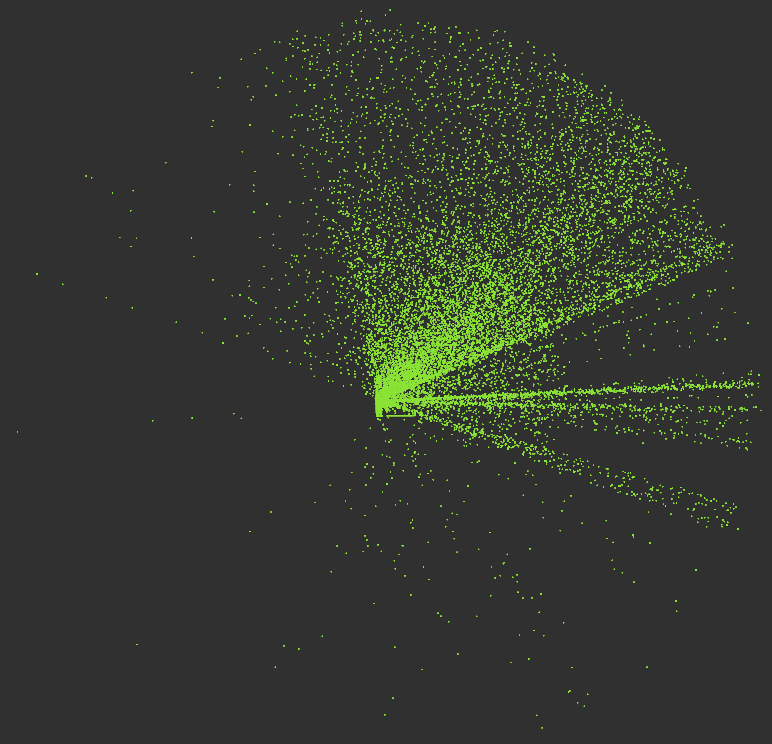
\includegraphics[width=\textwidth]{img/bosch/pandar40.png}
		\caption{HESAI's Pandar40 data scatter plot.}
		\label{fig:bosch-pandar40}
	\end{subfigure}
	\qquad
	\begin{subfigure}[t]{0.45\textwidth}
		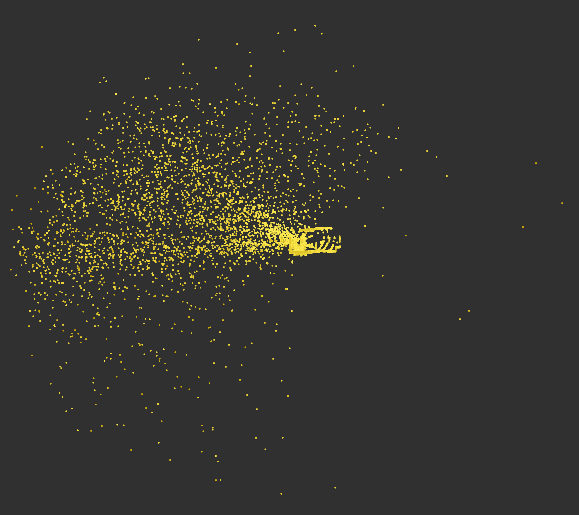
\includegraphics[width=\textwidth]{img/bosch/vlp16-test1.png}
		\caption{Velodyne's VLP-16 data scatter plot}
		\label{fig:bosch-vlp16-1}
	\end{subfigure}
	\caption{Scatter plot of the data gathered by HESAI's Pandar40, (\subref{fig:bosch-pandar40}), and Velodyne's VLP-16, (\subref{fig:bosch-vlp16-1}). The measurements are plotted only on the X-Y plane, flatenning the height of the points. }
	\label{fig:bosch-pandar-vs-vlp16}
\end{figure}

We also analyze the results from the second VLP-16bag file, and compare with the first, on figure~\ref{fig:bosch-vlp16-comparison}. The previous shown data, on figure~\ref{fig:bosch-vlp16-1} is shown in yellow and the second dataset in blue. On the center, the room can be seen, and the data, independently of the bag file, seems to have the same dispersion and directionality.

\begin{figure}[ht!]
	\centering
	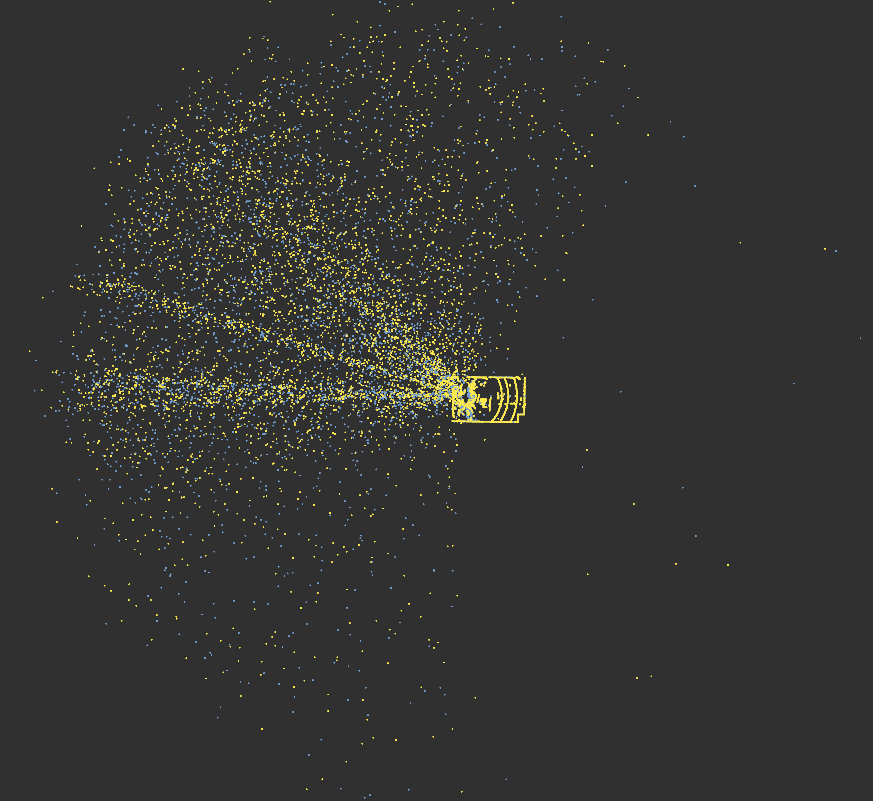
\includegraphics[scale=0.33]{img/bosch/vlp16-tests-overlaid.png}
	\caption{Scatter plot of the \ac{ros} bags containing Velodyne's VLP-16 data, gathered under the same conditions with almost an hour of difference. Thee measurements are plotted only on the X-Y plane, flatenning the height of the points. Comparison between the grid and blue points shows a macro-correspondance }
	\label{fig:bosch-vlp16-comparison}
\end{figure}

Since the room had people moving and no data without interference is present, this dataset cannot be used for a refined analysis of the interference, since the approach and methods we devise suppose that the environment is static, in order for a ground truth model to be generated. Since we have no camera information, no object detection processing chain can be implemented (similar to Chapter~\ref{chapter:object-detection}). 

Our solution is then to quantize this outliers and trying to understand more about their behavior, which is the approach detailed on the next Section.


\section{Room Outliers Contabilization}
After the qualitative analysis of the previous Section on Bosch's dataset, from which we concluded that the \ac{lidar} interference appears to be directional and causes outliers outside of the room dimensions, this Section details the implementation and results of a quantitative approach to analyze the events described on phenomenon 2: \ac{lidar} measurements outside room dimensions.

To analyze the data, a \ac{ros} node, with both offline and online versions, was implemented. Offline operation implies that the node does not have real-time constraints, being capable of handling large \ac{ros} bag files and datasets. The main difference from the online operation, that as been used so far, is that the node does not require another node on the network to publish data for him (tipically, a \ac{ros} bag player or a device driver) and the \ac{ros} network does not need to be setup up and running. Instead, the node loads and parses the bag file, as fast as it can or as fast as it is instructed to, keeping its data private on its own program memory. This alternative permits processing large amounts of data and realizing complex analysis on it.

To quantify this inteference, the node only needs to know the room dimensions, which we considered to be the majorant and minorant of the room dimensions along each of the 3 cartesian axes. With it, it can determine the number of point cloud messages received, average number of points per message, absolute and relative number of outliers and inliers. To account for some noise on the data, to the room limits dimensions, a 5\% tolerance is applied. 

An outlier is a point that is not contained within the room dimensions, in all three Cartesian coordinates, considering also the tolerance scaling. Given a point under classification, $P$, and define the tolerance as $t$, equation~\ref{eq:box-outlier-condition} describes the mathematical decision applied to determine if that point cloud point is an inlier or an outlier.

\begin{equation}
	\label{eq:box-outlier-condition}
	\begin{cases}
		\begin{aligned}
			\text{inlier}, \qquad \text{if } P \in & [\min(x) \cdot t, \max(x) \cdot t] \cup [\min(y) \cdot t, \max(y) \cdot t]  \\
																						&					 \cup [\min(z) \cdot t, \max(z) \cdot t] 
		\end{aligned} \\
		\text{outlier}, \qquad \text{otherwise}
	\end{cases}
\end{equation}

Despite this analysis not accounting for the possible interference inside the room dimensions, this interference model intends to measure what, to the ``naked eye'', is clearly an erroneous measure, caused by \ac{lidar} interference: measurements outside the physical dimensions of the room where the \acp{lidar} are located. Since the possible interference inside the room dimensions is not considered, we can view this metric as a minorant for the \ac{lidar} interference.


\subsection{Bosch Dataset}
To determine the room dimensions on Bosch dataset, we display the data on \texttt{RViz} and then use the selection tool to determine the maximum and minimum value on each axis that defines the room dimensions. This process is manual, and prone to error, specially since on this dataset, the \ac{lidar} axes are not oriented with the room\footnote{We can say that the \ac{lidar} axes are oriented with the room when a straight wall was one of its coordinates fixed on the \ac{lidar} coordinate frame, i.e., for every wall, there a \ac{lidar} axis that is parallel with the normal defined by the plane of the wall.} After determining such parameters, the data is analyzed and the results are presented on table~\ref{tab:bosch-dataset-stats}.

\begin{table}[!ht]
	\centering
	\renewcommand{\arraystretch}{1.2}
	\begin{tabular}{@{}llC{2cm}C{2.5cm}C{3.5cm}@{}}
		\toprule
		\multicolumn{2}{l}{Test Scenario} & \# \ac{lidar} messages & Average Points Per Message &  Normalized number of interferer points \\
			\midrule
		\multicolumn{2}{l}{\textit{Velodyne VLP-16}} & & & \\ 
		\phantom{ab} & \SI{5}{\hertz}  & 80  & 45582.3 & $1.10\E^{-3}$ \\ 
								 & \SI{10}{\hertz} & 199 & 22849.8 & $1.44\E^{-3}$ \\ 
		\midrule
		\multicolumn{2}{l}{\textit{HESAI Pandar40}} & & &  \\ 
		\phantom{ab} & \SI{20}{\hertz} & 406 & 25642.5 & $2.14\E^{-3}$ \\
		\bottomrule
	\end{tabular}
	\caption{Statistics of Bosch interference dataset. Room dimensions were manually determining from the interference dataset by selecting the points that correspond to the maximum and minimum value alongside the axis.}
	\label{tab:bosch-dataset-stats}
\end{table}

On Bosch's experimental setup, we can conclude that between one to two outliers outside of the room limits are expected for every 1000 points of data. These results offer a peak into \ac{lidar} interference, but we must restrain ourselves from premature conclusions.

Relatevely speaking, Pandar40 seems to have an higher presence of outliers than VLP-16, and data seems to suggest that an higher rotation speed increases the occurence of ``outside of the room dimensions'' outliers. However, the data diversity is reduced and the data that is available has low statiscally significance, since the number of tests is small and the duration of each of the bag files is smaller than \SI{20}{\second}.

We also need to consider that the room limits were manually determined, therefore these results are more prone to be affected by human error, which may be causing \ac{lidar} measurements inside of the room dimensions, inliers, to be considered erroneous and marked as outliers. Since the \ac{lidar} axes were also not oriented with the room, the errors are more likely. Also, the two \acp{lidar} are extremely close to each (less than 0.5\% of their measurement range, i.e., \SI{0.5}{\meter} and on the top of a table, which causes, at that distance, the lower beams of one \ac{lidar} to be reflected onto the other \ac{lidar}. 

Despite no conclusive veridects can be extracted from this data, we can affirm that the conditions under which this dataset is taken fosters the occurence of mutual \ac{lidar} interference, biasing the data by creating laboratorial scenarios difficult to happen on self-driving cars. We are also not sure if the higher number of interference on the HESAI Pandar40 is because it has more lasers or because Velodyne VLP-16 as more ``protection'' against interference\footnote{Velodyne as been working on this are. See the Release Notes on~\cite{vlp16}.}. 

\subsection{Our Experimental Dataset}
For our experimental dataset, we can automate the determination of the room dimensions from the data, since we have measurements of the test environments without interference. Therefore, the previous uncertanties regarding the manual determination of room limits are not present anymore. To automate the process, we developed a \ac{ros} node that parses a ground truth bag file and determines the room dimensions, considering the minorant and majorant points of the point cloud, , on the \ac{lidar} coordinate frame. 

As stated on Sub-section~\ref{subsec:lidar-interference:parameters-under-test}, 5 parameters under test are varied on our dataset, on \ac{irislab} facilities. The data gathered is analyzed and the results, for each of the parameters, are presented below, with the exception of the rotation speed.


Changing the rotation speed would require acessing HESAI's Pandar40 webserver, through an Ethernet conection, to configure its rotation speed~\cite{Pandar40UserGuide}. This attempts, however, were unfruitful, despite the several \ac{ros} drivers used, including official \ac{sdk} from HESAI\cp. Alternatively, VLP-16 rotation speed could be changed, instead, but we wanted the victim operation parameters to be constant at all time. Therefore, we opt to abandon the acquisition of interference data when the two \acp{lidar} operate at a different rotation speed.

\subsubsection{Distance}
The distance parameter was varied from \SIrange{1}{12}{\meter}, with steps of \SI{1}{\meter}. While varying the interferer position, the victim's \ac{lidar} remain unchanged. The interferer height was keept constant and ensuring that the \acp{lidar} optical center was at approximately the same height, with their relative orientation kept at approximately \SI{0}{\degree}.

The normalized number of outliers, with regard to the number of received points, is visualized on the bar chart on figure~\ref{fig:box-filter-outliers-distance}, for all the distances. The range of outliers varies from $10^{-7}$ to $10^{-5}$, significantly different from the results on Bosch's dataset, which were all on the order of magnitude of $10^{-3}$.

\begin{figure}[!ht]
	\centering
	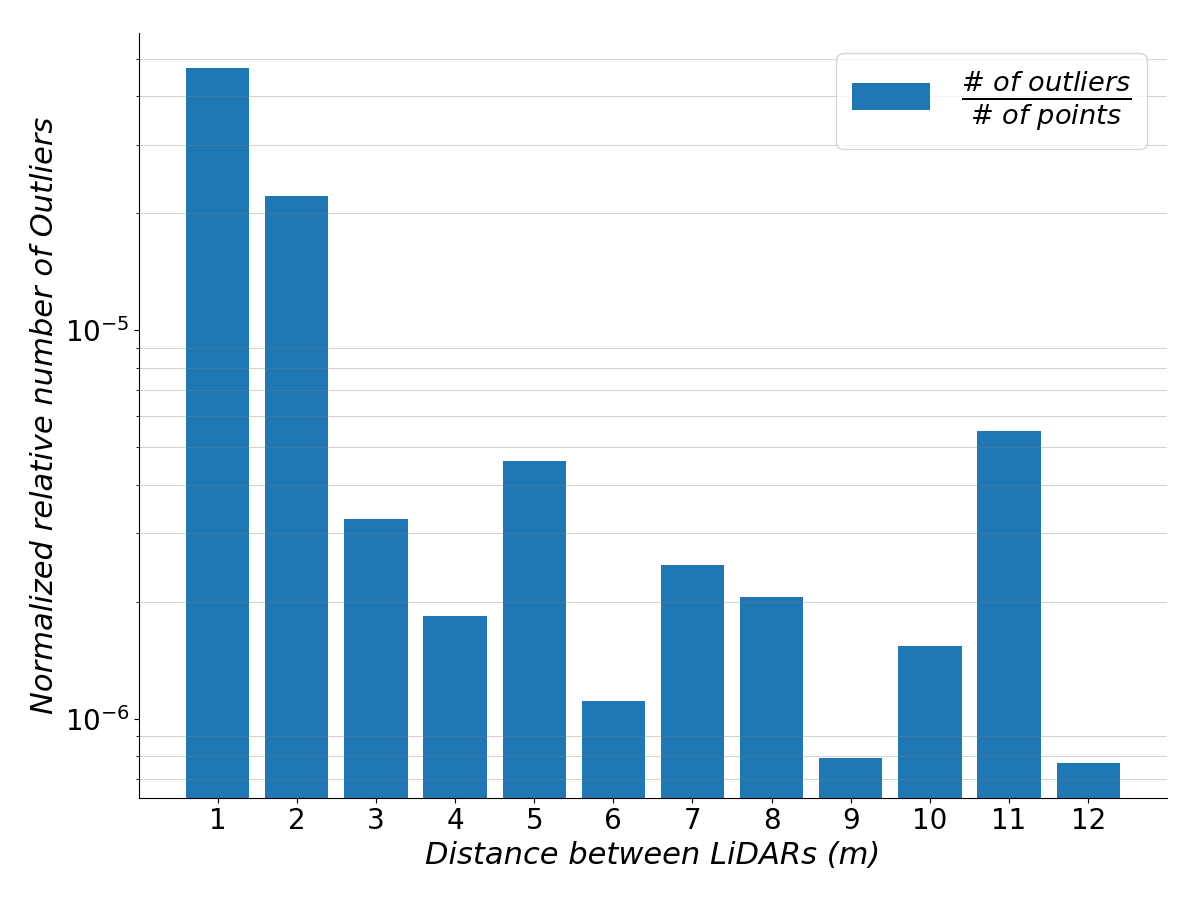
\includegraphics[width=0.8\textwidth]{img/lidar-interference/box-filtering/interference-box-filter-outliers-distance.png}
	\caption{Outlier contabilization when the parameter under test is the distance between the two \acp{lidar}. The outlier contabilization method is detailed on euqation~\ref{eq:box-outlier-condition}.}
	\label{fig:box-filter-outliers-distance}
\end{figure}

Despite the data not revelaing any perceivable patterns, there is a tendency for the higher values of outliers to occur for a closer distance between the \acp{lidar}. Note that this results do not indicate that the interference is higher the shorter the distance, but that the interference causes an higher number of points to be outside of the room dimensions if the two \acp{lidar} are closer. 

\subsubsection{Height}
Due to the \ac{lidar} photoreceptors and lasers orientation and internal organization, there are, theoretical, relative positioning and orientation between the two \acp{lidar} that either minize the interference or potentiate it. No theoretical analysis of such relations was carried, due to its impracticality: the application of such results to an extent it would benefit this research, i.e., gathering data under positions of maximum and minimum interference,  would require the alingment of a laser and a photoreceptor, whose position is only known approximatted, in free space of two different rotating devices.

For a fixed distance, our goal was to understand if variations of several orders of magnitude occurred when the relative height between the devices changed, which could hint on the relevance of the relative positioniung between the \acp{lidar} and its impact on the \ac{lidar} interference behaviour.

Figure~\ref{fig:box-filter-outliers-height} shows our analyzes of this parameter by measuring the relative number of outliers outside the room dimensions. Height difference values, presented on the x axis of the bar chart, indicate the relative height between the HESAI and the Velodyne \acp{lidar}. The interferer \ac{lidar} was placed at a distance of \SI{4}{\meter} of the victim and their relative orientation was kept approximately at \SI{0}{\degree}.

\begin{figure}[!ht]
	\centering
	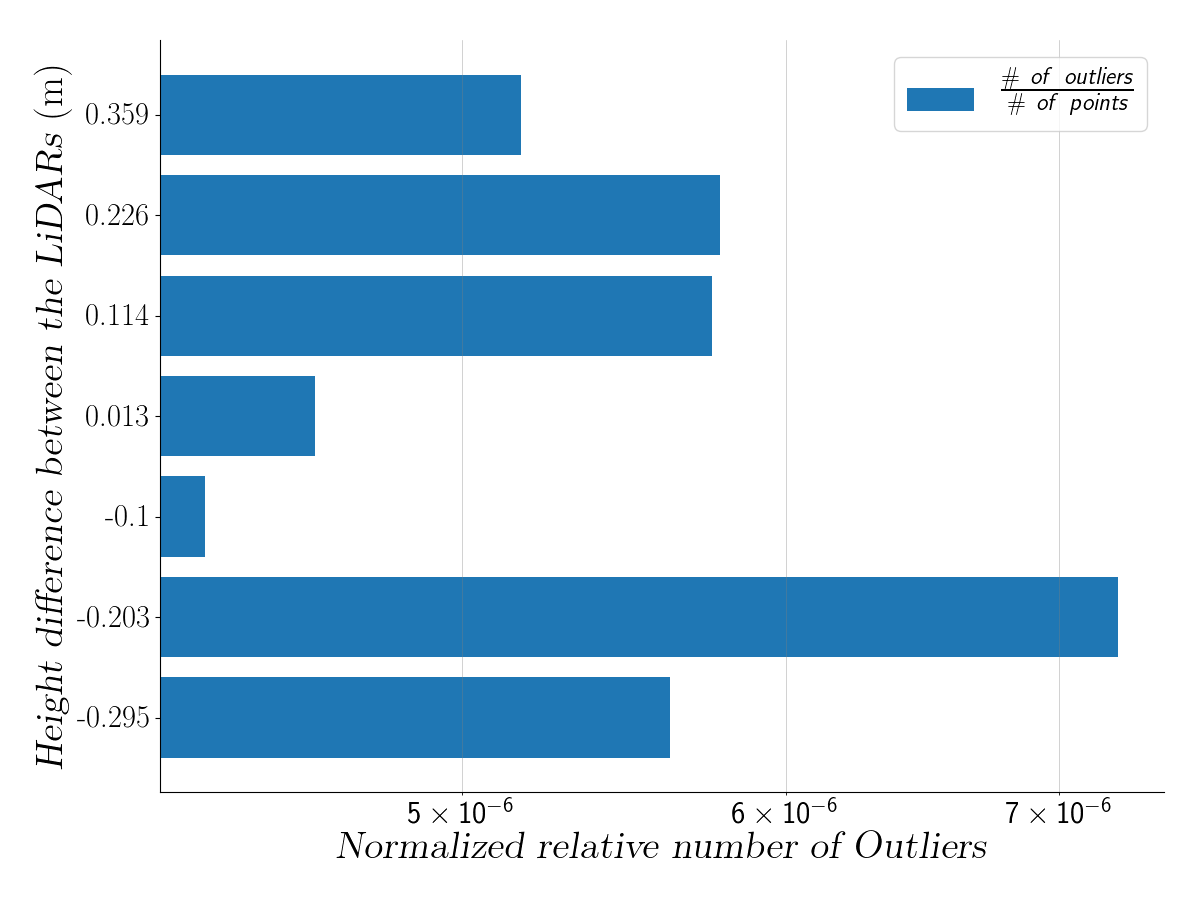
\includegraphics[width=0.8\textwidth]{img/lidar-interference/box-filtering/interference-box-filter-outliers-height.png}
	\caption{Outliers analyzes when the parameter under test is height. On the x axis, the height variation indicates the Pandar40 relative position in relation to the VLP-16 and is measured at their supposed optical centers.}
	\label{fig:box-filter-outliers-height}
\end{figure}

The results obtained are all on the same order of magnitude, $10^{-6}$, having a variation, between its maximum and its minimum of approximately 7 times. They show that when their optical center is aligned, the number of outliers is at its lower, but coherent with the results of figure~\ref{fig:box-filter-outliers-distance}: around $2\E^{-6}$. Despite the higher interference value occurring for a height difference of $\approx \SI{-0.2}{\meter}$, opting to place the interferer \ac{lidar} above or below the victim \ac{lidar} increases the number of outliers when comparing with the two \acp{lidar} being aligned. However, opting from above instead of below (or vice-versa), does not appear to have any significant advantage. 

\subsubsection{\acp{lidar} \ac{los} Obstruction}
To assess the impact of direct vs indirect interference on the number of outliers, we obstrcuted the \acf{los} between the two \acp{lidar} with a straight box. The goal of this obstruction is to block direct beams between the two \acp{lidar}, therefore eliminating direct \ac{lidar} interference. With this contraption, data is recorded at even distances between the two \ac{lidar}, with the obstacle placed in their middle distance. As expected, when the distance is increased between the two \acp{lidar}, the distance between each of them to the obstacle also increases, resulting in a smaller angular occupation of the \acp{lidar} \ac{fov} with the obstacle. Reducing the angular occupation potentially increases the number of rays that can cause indirect interference on the victim's \ac{lidar}. However, no actions were taken to further research on this premise, since \acp{lidar} interference behavior has not yet been fully understood.

On figure~\ref{fig:box-filter-outliers-LOS}, the outlier analysis under a scenario of \ac{los} between the \acp{lidar} is shown. When comparing with the results of the distance test, on figure~\ref{fig:box-filter-outliers-distance}, a reduction of one order of magnitude is noticeble on all distances except the outliers at a distance of \SI{8}{\meter} and \SI{12}{\meter}, on which the number of outliers remain approximately equal. 

\begin{figure}[!ht]
	\centering
	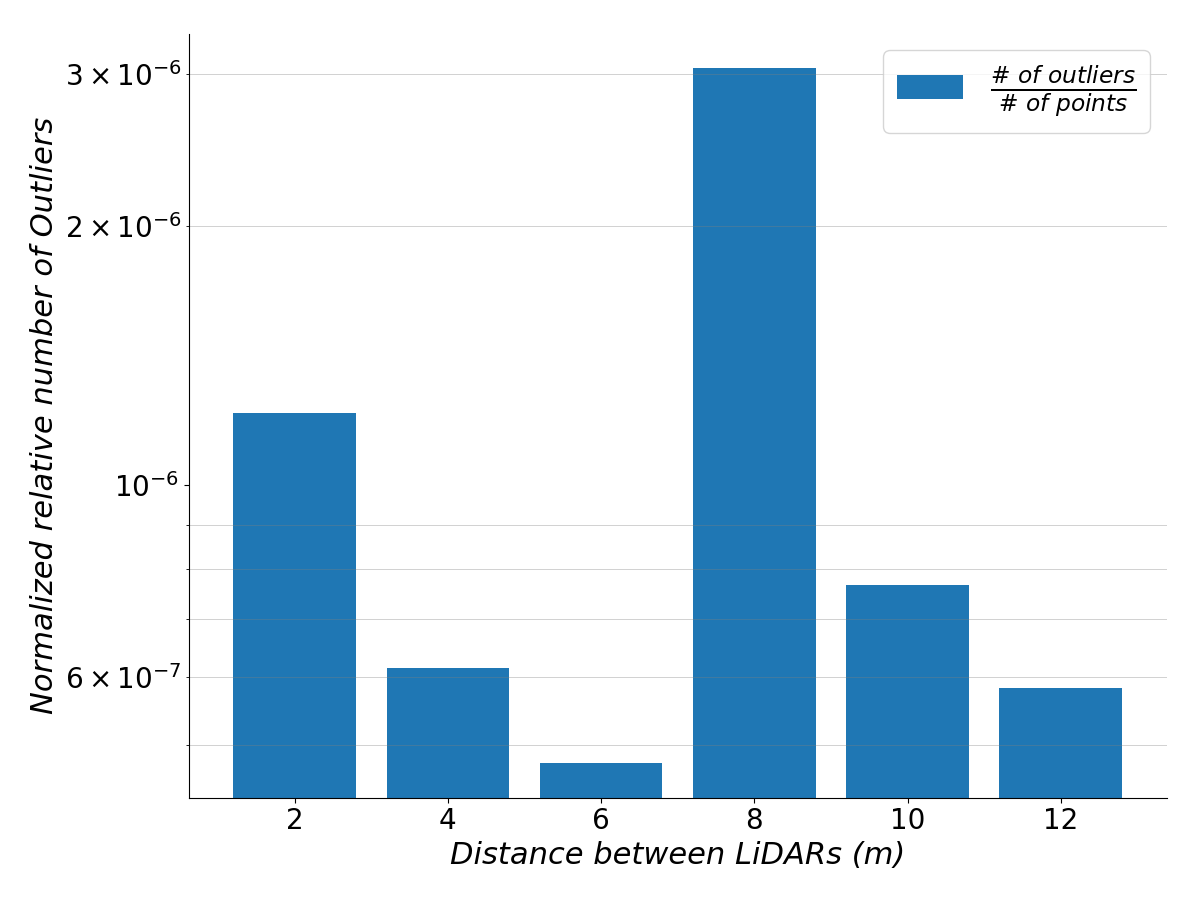
\includegraphics[width=0.8\textwidth]{img/lidar-interference/box-filtering/interference-box-filter-outliers-LOS.png}
	\caption{Box filtering applied to all the interference data where the distance was varied, with an obstacle obstructing the \acp{lidar} \ac{los}. The distance variation correspond to the even numbers from the distance test and the obstacle was always placed in between the two \ac{lidar}.}
	\label{fig:box-filter-outliers-LOS}
\end{figure}

Those findings leds us to believe that the most significant part of the outliers that are outside of the room are caused by direct interference. Two subsets of the graphics' data are monotonous decrescent: from \SIrange{2}{6}{\meter} and \SIrange{8}{12}{\meter}. Inside each of these subsets, the number of outliers reduces with the distance, but the behavior described on the distance test, were the major values of outliers occured on short distances, is not verified where. We are also led to believe that to short distances, direct interference predominates, reason why on the distance setup without \ac{los} obstruction, the number of outliers is higher to short distances than they are with \ac{los} obstruction.

\subsubsection{Relative orientation}
To comprehend if the orientation between the \acp{lidar} affects the number of outliers, the interferer \ac{lidar} orientation was changed, keeping their relative distance constant. Tests were perfomed with an angular step of \SI{30}{\degree}, creating 12 data points that are shown on figure~\ref{fig:box-filter-outliers-direction}.

\begin{figure}[!ht]
	\centering
	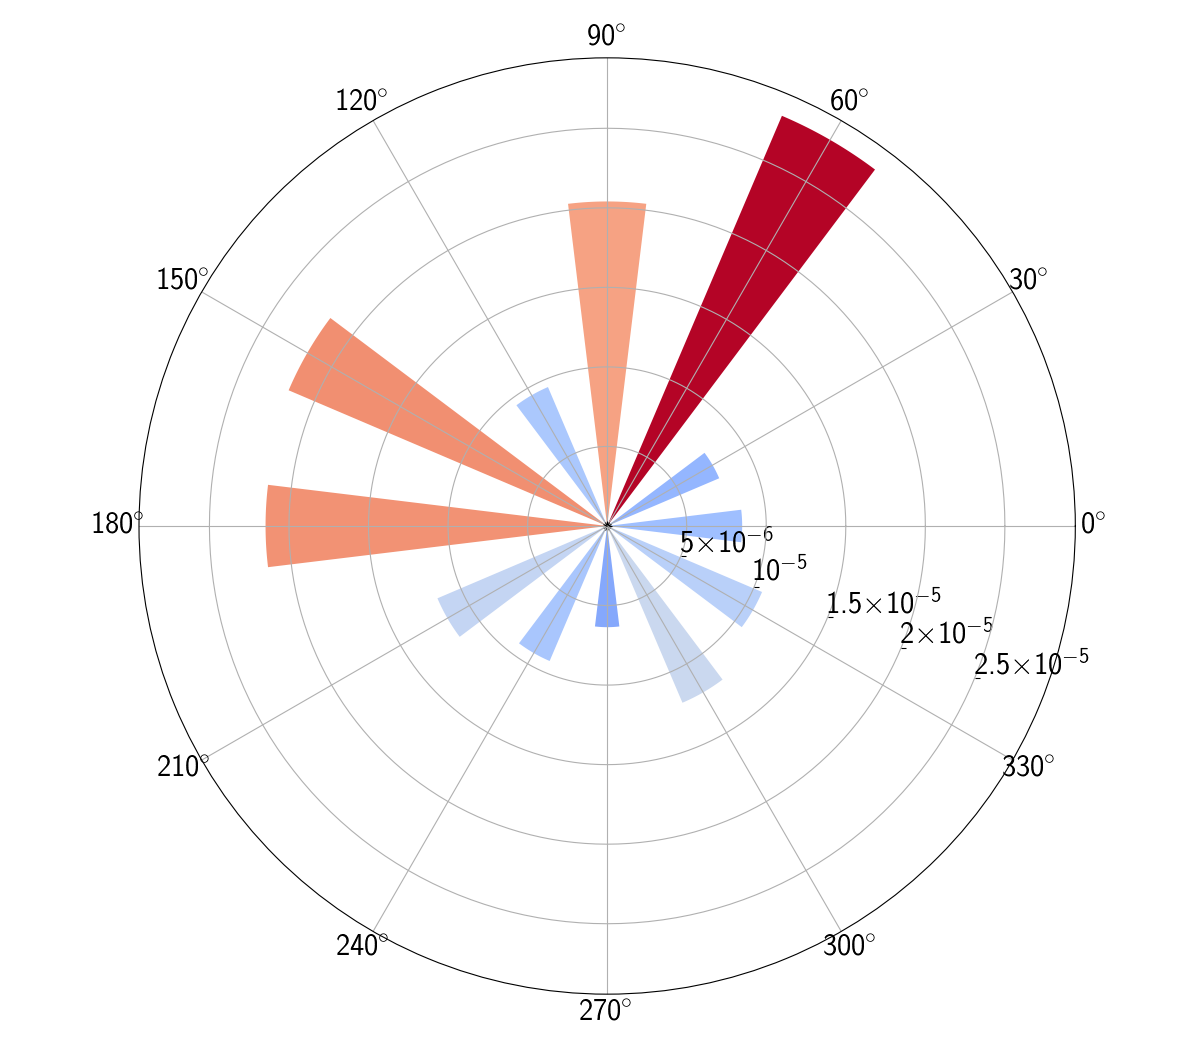
\includegraphics[width=0.5\textwidth]{img/lidar-interference/box-filtering/interference-box-filter-outliers-direction.png}
	\caption{Normalized number of outliers with regrad to the orientation between the \ac{lidar}. On this polar chart, the higher the bar, the higher the value of interference. With the exception of 4 angles (\SIlist[list-final-separator = {, }]{60; 90; 150; 180}{\degree}) is greater than the other angles by an order of magnitude ($10^{-6}$ vs $10^{-7}$).}
	\label{fig:box-filter-outliers-direction}
\end{figure}

The normalized number of outliers magnitude variation between the angular positions results on a relative number of outliers to one in a million points or to one in 10 million points. Some dependence with the relative \ac{lidar} orientation is present, with 4 angles, \SIlist[list-final-separator = {, }]{60; 90; 150; 180}{\degree}, having a normalized number of outliers one order of magnitude greater than the remaining 8 angles: $10^{-6}$ vs $10^{-7}$.

% Note: Writing this here would imply creating figures that show the directionatility of the data, i.e., play the rosbag files and accumulate them on Rviz. Alternatively, a point accumulator ros node ros node can be built ;)
%On figure~\ref{fig:bosch-pandar-vs-vlp16}, we see a clearly directionality of data and from our findings, there seem to be a small impact of the orientation between \acp{lidar}. As we have stated, the scatter plot represebntation seems to enfatize the problem of \ac{lidar} interference, making it seem more complex, when in reality, a heatmap should be used instead to represen, in order to plot the density.


\subsubsection{\ac{it} Dark Room}
\ac{it} 2 Dark Room test methodology differs from the one used on \ac{irislab}, since two parameters were varied simultaneous, instead of only one: distance and height. The relation between this data is presented on figure~\ref{fig:box-filter-outliers-it2}. Along its x-axis, distance is variated and on its y-axis, the relative height between the \acp{lidar} is changed.

\begin{figure}[!ht]
	\centering
	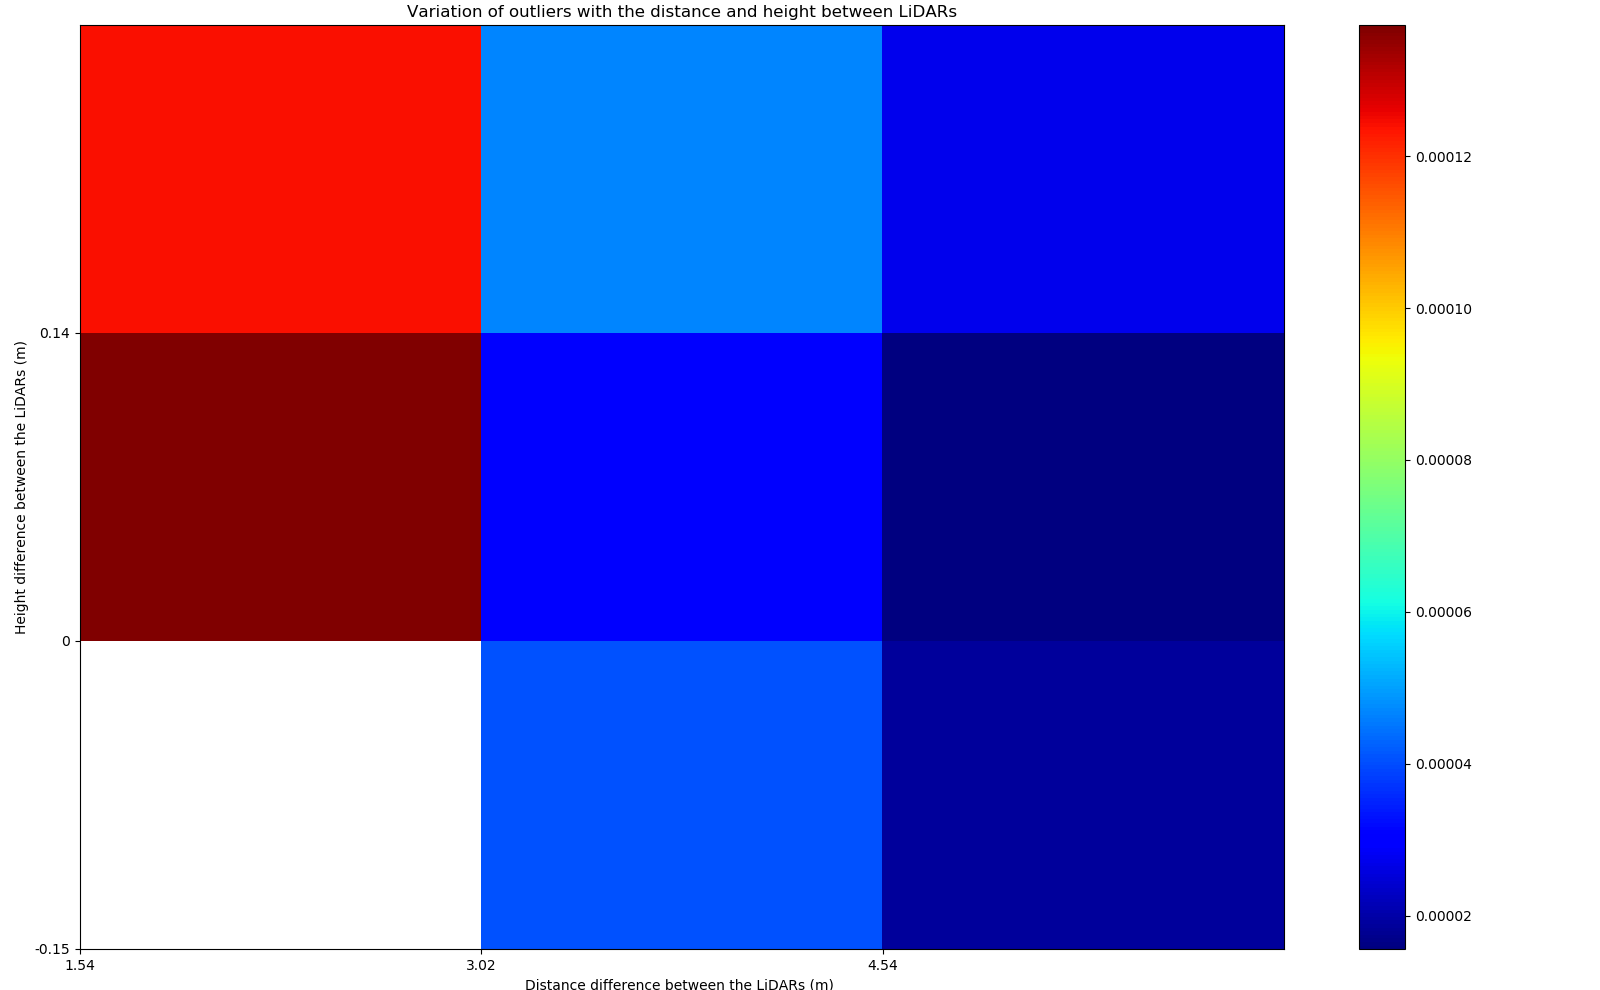
\includegraphics[width=0.8\textwidth]{img/lidar-interference/box-filtering/interference-box-filter-outliers-it2.png}
	\caption{\ac{it} 2 Dark Room results. Relative height and distance between the victim's and interferer \ac{lidar} were varied. Along the x-axis, distance variations between the \acp{lidar} are considered and on the y-axis, the height differences. The left bottom data point is blank due to data corruption.}
	\label{fig:box-filter-outliers-it2}
\end{figure}

The white square on the left bottom of the figure is empty because the bag file containing that data was corrupted during saving and data could not be recovered. From the image, we corroborate the previous results from the distance tests (figure~\ref{fig:box-filter-outliers-distance}): the closer the \acp{lidar} are, the higher the number of outliers. If the interferer \ac{lidar} is above the victim's \ac{lidar}, the number of outliers also increases slighty, when comparing with the other heights tested.

\section{Ground-Truth Generation}
\label{sec:lidar-interference:ground-truth}
To deepen our understanding of \ac{lidar} interference, the possibility that \ac{lidar} interference not only causes erroneous measures that are clearly outliers of the data, but also more subtle errors, possible similar to sensor noise, must be accepted. To test this premise, we need to compare the point clouds with interference with a known model of the environment, a ground-truth, that contains no interference.  

A ground truth model of the environment cane be a specific point cloud from all the data or can be generated by considering multiple point cloud frames, from interference-free data. The latter is preferred, since it has more chances of removing sensor noise from the data. Due to the lack of no viable alternatives on the \acl{sota}, we propose two algorithms for ground-truth generation, which are capable of fusing multiple point cloud frames from a bag file, generating a model that better resembles the real characteristics of the room.


\subsection{Frame Stitching}
\label{subsec:lidar-interference:frame-stitching}
Frame stitching consists on, given two point cloud frames, aligning a second point cloud frame with the first and then merge their data into a single point cloud frame. Iteratively perfoming this operation would create a single point cloud that progressevly contains the best estimation of the environment point cloud, using multiple point clouds.

To implement this, first the two frames to be stitched are filtered, using \ac{pcl}'s Voxel Grid filter, with a voxel edge length of \SI{5}{\centi\meter}. This step ensures the data density and spatial organization of the point clouds is similar, which yelds better results on the stitching process and also speeds it up, due to a reduction of the data points.

To stitch the two voxelized data frames together, an \ac{icp} algorithm is used. Our solution uses \ac{pcl} library and therefore, \ac{pcl}'s implementation of the \ac{icp} algorithm. \ac{icp} is an algorithm oriented to merge point cloud that have been acquired from different positions and only have some points in common. It performs the computation of the joint rotation and translation matrix, that transforms one point cloud coordinate frame to the others', aligning them. The computation of \ac{icp}'s transformation matrix uses \ac{svd} to compute the rotation and translation matrix that aligns the two point clouds.

On our case, \ac{icp} will align the two point clouds, that are taken from the same position, but whose data, due to the \ac{lidar} measurement noise, will not be equal. The parameters used for this algorithm are present on table~\ref{tab:frame-stitching-parameters}. On \ac{icp}'s algorithm, the correspondences to be considered for the statistical analysis of the \ac{icp}'s convergence must be smaller than \SI{2}{\centi\meter}. Three termination criterea for the algorithm exist and must be tuned:

\begin{enumerate}
	\item \textbf{Maximum number of iterations:} If the algorithm reaches this number of interations without converging, it stops and returns an error, indicating that it as not converged.
	\item \textbf{Transformation Epsilon:} When iterating to refine the transformation computed internally, it terminates if the difference between the current and last transformation matrix is smaller than this parameter;
	\item \textbf{Euclidian Difference Fitness Epsilon:} When iterating, terminates if the Euclidian errors (distance between the alinged source and target point cloud) is smaller than this threshold.
\end{enumerate}


\begin{table}[H]
	\centering
	\renewcommand{\arraystretch}{1.2}
	\begin{tabular}{@{}lp{8cm}c@{}}
		\toprule
		\multicolumn{2}{l}{Specification} & Value \\
			\midrule
		\multicolumn{2}{l}{\textit{Voxel Filter}} & \\ 
		\phantom{ab} & Voxel edge length & \SI{5}{\centi\meter} \\ 
		\midrule
		\multicolumn{2}{l}{\textit{\ac{pcl}'s \ac{icp}}} &  \\ 
		\phantom{ab} & Maximum Correspondences Distance & \SI{2}{\centi\meter} \\
								 & Maximum Number of Iterationt & 50 \\
								 & Transfomration Epsilon & $1\E^{-8}$ \\
								 & Euclidian Difference Fitness Epsilon & \SI{5}{\centi\meter} \\
		\bottomrule
	\end{tabular}
	\caption{Parameter values used on the Frame Stitching algorithm, for the Voxel Grid and \ac{icp}.}
	\label{tab:frame-stitching-parameters}
\end{table}

When it finishes computing the ground truth point cloud, the \ac{ros} node that implements this algorithm saves the ground truth \ac{lidar} point cloud on a \ac{pcd} file.

This solution was some caveats, since it considers one of the point cloud frames to be the source to which all the other frames must be matched, i.e, the second frame is stitched to match the first frame, and the third frame is stitched to match the result of the filtered second and first frame, and so on. Also, despite \ac{pcl} being a templated library that can work with whatever point types are defined by the user, \ac{pcl} \ac{icp} implementation destroys the laser ID information that point clouds obtained from the VLP-16 contain, which limits the possibilities for interference analysis. 


\subsection{Frame Registration}
\label{subsec:lidar-interference:frame-registration}
Frame Registration is a ground truth model generation algorithm based on an organized point cloud data structure, which was primarly developed for \ac{lidar} interference analysis, but was later generalized to be used for ground truth model generation.

An organized point cloud is a data structure similar to the point cloud previously used, but its two-dimensional organization contains information about the adjacent points of a given point. This spacial organiztion mimics a depth image, with rows and columns, but differs from the latter since the data containing on each index of the data matrix is not only depth, but instead a point cloud point.

Our implementation, which extends \ac{pcl}'s organized point data structure, is a generic and templated data structure, that can suport not only point cloud points as its basis data type. This peculiarity allows the usage of abstract point cloud containers, which contain point cloud data, but also other metrics, for every index of the data matrix. For ground truth generation, the container developed holds a vector of points cloud points, to store the registered point cloud points for that index. Fields for the intensity, position and distance are also available, both for the average value and the variance.

The ground truth technique developed computes, for every point of all the point cloud frames on a bag file, the index (row and column) to which that point belongs on the organized point cloud structure, and appends it to the point vector of that index container. On spherical coordinates, the point row index corresponds to its azimuthal angle and the column to its polar angle. On Velodyne \ac{lidar}'s, the polar angle is determined by the laser ID from which the pulse was fired and the azimuthal angle can be determined by equation~\ref{eq:azimuthal-angle}, from which the $x$ and $y$ coordinates are known from the point data. From the azimuthal angle, the azimuthal index of the matrix can be found by dividing the azimuthal angle with the angular step of the VLP-16, as shown in equation~\ref{eq:azimuthal-angle-index}

\begin{equation}
	\label{eq:azimuthal-angle}
	\theta = \arctan\left(\frac{y}{x}\right) \cdot \frac{\SI{180}{\degree}}{\pi}
\end{equation}

\begin{equation}
	\label{eq:azimuthal-angle-index}
	\theta_{\text{index}} = \frac{\theta}{\text{VLP-16 angular step}} = \frac{\theta}{\SI{0.2}{\degree}} 
\end{equation}

After registering the full point cloud data, the ground truth model can be generated. Our implementation uses an average estimator that iterates over all the indexes of the matrix, computing the average point cloud coordinate using the vector of points registered, which will be the ground truth model coordinates. Alongise this position value for the ground truth model, ithis estimator also computes the variance and average value of the point of vectors distance and intensity.



\subsection{Comparison}

%Direct interference (on Kim's experimental setup and hardware) is likely to saturate the receptor of the interfered \ac{lidar}, which may or may not be considered a valid measurement by the hardware and may discarded by the driver before being registered;

\section{Voxel-ize Analysis}
\subsection{Theoretical Principle}
\subsection{Implementation}
\subsection{Results}
\subsubsection{Distance}
\subsubsection{Height}
\subsubsection{\acp{lidar} \ac{los} Obstruction}
\subsubsection{Direction}

\section{Point-to-Point Analysis}
\subsection{Theoretical Principle}
\subsection{Implementation}
\subsection{Results}
\subsubsection{Distance}
\subsubsection{Height}
\subsubsection{\acp{lidar} \ac{los} Obstruction}
\subsubsection{Direction}

\section{Interference on \acp{roi}}

\section{\acl{sota} Comparison}
Note that, for all the data presented, there are two considerations that are not addressed. First, as far as we know, there are no certanties of the extent of likelyness that direct \ac{lidar} interference can saturate the receptor of the victim's \ac{lidar}, which may or may not be considered a valid measurement by the hardware, and may or may not be discarded by the driver before being registered. Also, since the \ac{lidar}'s hardware and the driver software impose a maximum on the distance at which a point can be measured, our mecanism for data reception can, perhaps, be removed on the hardware or software level. Our experiments had led us to thinkering about these problems, but no action was taken to address them.
